\documentclass[12pt,a4paper]{article}

%\usepackage[left=1.5cm,right=1.5cm,top=1cm,bottom=2cm]{geometry}
\usepackage[in, plain]{fullpage}
\usepackage{array}
%\usepackage{../../pas-math}
\usepackage{../../moncours}



%-------------------------------------------------------------------------------
%          -Packages nécessaires pour écrire en Français et en UTF8-
%-------------------------------------------------------------------------------
\usepackage[utf8]{inputenc}
\usepackage[frenchb]{babel}
%\usepackage{numprint}
\usepackage[T1]{fontenc}
%\usepackage{lmodern}
\usepackage{textcomp}
\usepackage[french, boxed]{algorithm2e}
\usepackage{hyperref}


%-------------------------------------------------------------------------------

%-------------------------------------------------------------------------------
%                          -Outils de mise en forme-
%-------------------------------------------------------------------------------
\usepackage{hyperref}
\hypersetup{pdfstartview=XYZ}
%\usepackage{enumerate}
\usepackage{graphicx}
\usepackage{multicol}
\usepackage{tabularx}
\usepackage{multirow}
\usepackage{color}
\usepackage{eurosym}


\usepackage{anysize} %%pour pouvoir mettre les marges qu'on veut
%\marginsize{2.5cm}{2.5cm}{2.5cm}{2.5cm}

\usepackage{indentfirst} %%pour que les premier paragraphes soient aussi indentés
\usepackage{verbatim}
\usepackage{enumitem}
\usepackage{booktabs}
\usepackage[usenames,dvipsnames,svgnames,table]{xcolor}

\usepackage{variations}

%-------------------------------------------------------------------------------


%-------------------------------------------------------------------------------
%                  -Nécessaires pour écrire des mathématiques-
%-------------------------------------------------------------------------------
\usepackage{amsfonts}
\usepackage{amssymb}
\usepackage{amsmath}
\usepackage{amsthm}
\usepackage{tikz}
\usepackage{xlop}
\usepackage[output-decimal-marker={,}]{siunitx}
%-------------------------------------------------------------------------------

%-------------------------------------------------------------------------------
%                  -Nécessaires pour écrire des formules chimiquess-
%-------------------------------------------------------------------------------

\usepackage[version=4]{mhchem}

%-------------------------------------------------------------------------------
% Pour pouvoir exploiter les fichiers directement dans beamer
\newcommand{\pause}{\ }
%-------------------------------------------------------------------------------
%                    - Mise en forme avancée
%-------------------------------------------------------------------------------

\usepackage{ifthen}
\usepackage{ifmtarg}


\newcommand{\ifTrue}[2]{\ifthenelse{\equal{#1}{true}}{#2}{$\qquad \qquad$}}

%\newcommand{\kword}[1]{\textcolor{red}{\underline{#1}}}
%-------------------------------------------------------------------------------

%-------------------------------------------------------------------------------
%                     -Mise en forme d'exercices-
%-------------------------------------------------------------------------------
%\newtheoremstyle{exostyle}
%{\topsep}% espace avant
%{\topsep}% espace apres
%{}% Police utilisee par le style de thm
%{}% Indentation (vide = aucune, \parindent = indentation paragraphe)
%{\bfseries}% Police du titre de thm
%{.}% Signe de ponctuation apres le titre du thm
%{ }% Espace apres le titre du thm (\newline = linebreak)
%{\thmname{#1}\thmnumber{ #2}\thmnote{. \normalfont{\textit{#3}}}}% composants du titre du thm : \thmname = nom du thm, \thmnumber = numéro du thm, \thmnote = sous-titre du thm

%\theoremstyle{exostyle}
%\newtheorem{exercice}{Exercice}
%
%\newenvironment{questions}{
%\begin{enumerate}[\hspace{12pt}\bfseries\itshape a.]}{\end{enumerate}
%} %mettre un 1 à la place du a si on veut des numéros au lieu de lettres pour les questions 
%-------------------------------------------------------------------------------

%-------------------------------------------------------------------------------
%                    - Mise en forme de tableaux -
%-------------------------------------------------------------------------------

\renewcommand{\arraystretch}{1.7}

\setlength{\tabcolsep}{1.2cm}

%-------------------------------------------------------------------------------



%-------------------------------------------------------------------------------
%                    - Racourcis d'écriture -
%-------------------------------------------------------------------------------
%Droites
\newcommand{\dte}[1]{$(#1)$}
\newcommand{\fig}[1]{figure $#1$}
\newcommand{\sym}{symétrique}
\newcommand{\syms}{symétriques}
\newcommand{\asym}{axe de symétrie}
\newcommand{\asyms}{axes de symétrie}
\newcommand{\seg}[1]{$[#1]$}
\newcommand{\monAngle}[1]{$\widehat{#1}$}
\newcommand{\bissec}{bissectrice}
\newcommand{\mediat}{médiatrice}
\newcommand{\ddte}[1]{$[#1)$}


% Angles orientés (couples de vecteurs)
\newcommand{\aopp}[2]{(\vec{#1}, \vec{#2})} %Les deuc vecteurs sont positifs
\newcommand{\aopn}[2]{(\vec{#1}, -\vec{#2})} %Le second vecteur est négatif
\newcommand{\aonp}[2]{(-\vec{#1}, \vec{#2})} %Le premier vecteur est négatif
\newcommand{\aonn}[2]{(-\vec{#1}, -\vec{#2})} %Les deux vecteurs sont négatifs

%Ensembles mathématiques
\newcommand{\naturels}{\mathbb{N}} %Nombres naturels
\newcommand{\relatifs}{\mathbb{Z}} %Nombres relatifs
\newcommand{\rationnels}{\mathbb{Q}} %Nombres rationnels
\newcommand{\reels}{\mathbb{R}} %Nombres réels
\newcommand{\complexes}{\mathbb{C}} %Nombres complexes


%Intégration des parenthèses aux cosinus
\newcommand{\cosP}[1]{\cos\left(#1\right)}
\newcommand{\sinP}[1]{\sin\left(#1\right)}


%Probas stats
\newcommand{\stat}{statistique}
\newcommand{\stats}{statistiques}


\newcommand{\homo}{homothétie}
\newcommand{\homos}{homothéties}


\newcommand{\mycoord}[3]{(\textcolor{red}{\num{#1}} ; \textcolor{Green}{\num{#2}} ; \textcolor{blue}{\num{#3}})}
%-------------------------------------------------------------------------------

%-------------------------------------------------------------------------------
%                    - Mise en page -
%-------------------------------------------------------------------------------

\newcommand{\twoCol}[1]{\begin{multicols}{2}#1\end{multicols}}


\setenumerate[1]{font=\bfseries,label=\textit{\alph*})}
\setenumerate[2]{font=\bfseries,label=\arabic*)}


%-------------------------------------------------------------------------------
%                    - Elements cours -
%-------------------------------------------------------------------------------

%Correction d'exercice
\newcommand{\exoSec}[2]{\subsection*{Exercice #1 page #2}}
%-------------------------------------------------------------------------------
%                    - raccourcis d'écriture -
%-------------------------------------------------------------------------------

%Mise en évidence de termes clés
\newcommand{\mykw}[1]{\textcolor{red}{\underline{\textbf{#1}}}}

%Exercices
\newcommand{\exo}[2]{exercice #1 page #2}
\newcommand{\Exo}[2]{Exercice #1 page #2}

\renewcommand{\pause}{\ }

%Intervalles
\newcommand{\interOO}[2]{$]$#1 , #2$[$}
\newcommand{\interOF}[2]{$]$#1 , #2$]$}
\newcommand{\interFO}[2]{$[$#1 , #2$[$}
\newcommand{\interFF}[2]{$[$#1 , #2$]$}



\begin{document}
	
	
\chap[num=14, color=blue]{\small Quelle est la composition de l'air ?}{Olivier FINOT, \today }	

\section{L'air dans l'atmosphère}

\begin{myact}{1 page 124}
	\begin{enumerate}
		\item Non les glaçons n'ont pas la forme du récipient qui les contient.\pause
		\item Le liquide obtenu lorsque les glaçons ont fondu a la forme du récipient.\pause
		\item La surface libre du liquide est plane.\pause
		\item On peut saisir un glaçon avec ses doigts, mais pas de l'eau liquide.\pause
		\item Lorsqu'il est placé dans des récipients de forme différentes, un solide conserve sa forme.\pause
		\item Un solide a une forme propre parce qu'elle ne change pas.\pause
		\item Un liquide placé dans dans des récipients de formes différentes prend la forme de ces récipients.\pause
		\item Le fil à plomb indique la direction verticale, donc le petit côté de l'équerre indique la direction horizontale. On en déduit que la surface libre d'un liquide au repos est horizontale.
	\end{enumerate}
\end{myact}

\begin{mybilan}
	\begin{itemize}
		\item Un \kw{solide} a une \kw{forme propre} qui ne change pas, on peut le saisir.
		\item Un \kw{liquide} prend la \kw{forme du récipient} qui le contient.
		\item La surface d'un liquide en contact avec l'air est sa \kw{surface libre}.
		\item Au repos, cette surface libre est \kw{plane et horizontale}.
	\end{itemize}	   
\end{mybilan}

%\begin{myexos}
%	\twoCol{
%	\begin{itemize}
%		\item \exo{1}{20}
%	\end{itemize}}
%\end{myexos}

\section{Composition de l'air}

\begin{myact}{2 page 125}
	\begin{enumerate}
		\item Lorsque l'eau bout, il se forme de la vapeur dans l'erlenmeyer.\pause
		\item La vapeur d'eau emprisonnée dans l'erlenmeyer occupe tout l'espace disponible.\pause
		\item Quand les deux erlenmeyers sont en communication, on voit apparaître de la buée sur la paroi, car la vapeur est montée dans le deuxième erlenmeyer.\pause
		\item Après la mise en communication, la vapeur occupe l'espace des deux erlenmeyers.\pause
		\item Lorsque l'on appuie sur le piston, le volume d'air contenu dans la seringue fermée diminue.\pause
		\item Non, la vapeur d'eau n'a pas de forme propre.\pause
		\item La vapeur d'eau est expansible car lorsque l'on ajoute le second erlenmeyer, elle l'occupe en plus du premier.\pause
		\item Lorsque l'on appuie sur le piston de la seringue fermée, le volume d'air diminue, l'air est donc compressible.
	\end{enumerate}
\end{myact}

\begin{mybilan}
	Pour décrire la vitesse d'un objet en mouvement, on utilise trois caractéristiques :
	\begin{itemize}
		\item la \kw{direction} (horizontale, verticale ou oblique), tangente à la trajectoire;
		
		\item le \kw{sens}, celui du mouvement (vers la gauche, vars la droite, vers le haut etc.);
		
		\item la \kw{valeur} exprimée m/s (ou km/h ou autre).
		
		Si le mouvement est uniforme, la relation \kw{$ v = \dfrac{d}{\Delta t} $}, permet de relier la vitesse de l'objet, la distance parcourue et la durée du parcours avec :
		\begin{itemize}
			\item d : distance parcourue en mètre (m)
			\item $\Delta t$ :durée du trajet en seconde (s)
			\item v : vitesse en mètre par seconde (m/s).
		\end{itemize}
	\end{itemize}



\end{mybilan}



\begin{myexos}
	\twoCol{
	\begin{itemize}
		\item \exo{610}{21}
		\item \exo{9}{21} (sans question d)
		\item \exo{13}{22}
		\item \exo{17}{23}
		\item \exo{19}{23}
	\end{itemize}}
\end{myexos}

\section{Gaz et fumées}

\begin{myact}{3 page 126}
	\begin{enumerate}
		\item Au début de l'expérience le tube à essais contient de l'eau.\pause
		\item Au cours de l'expérience, dans le tube à essais des bulles apparaissent et le niveau de l'eau diminue.\pause
		\item Le bain-marie est à \num{57.6} °C.\pause
		\item Non il n'est pas nécessaire de faire beaucoup chauffer l'eau pétillante pour en récupérer le gaz.\pause
		\item Au cours de l'expérience, l'eau des tubes à essais est remplacée par du gaz.\pause
		\item Le gaz dégagé est récupéré par déplacement d'eau car il prend la place de l'eau contenue dans le tube à essais.\pause
		\item Pour récupérer le gaz contenu dans le l'eau pétillante on peut l'agiter  ou la chauffer.
	\end{enumerate}
\end{myact}

\begin{mybilan}
	
	\twoCol{
	\begin{center}
		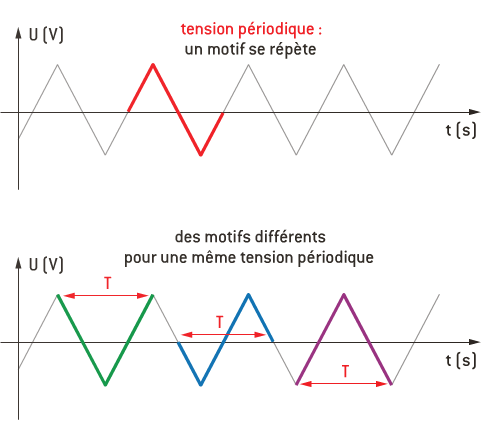
\includegraphics[scale=0.7]{bilan3}
	\end{center}

	\begin{itemize}
		\item Une tension est \kw{périodique} lorsque ses \kw{variations se répètent} identiques à elles mêmes au cours du temps. 
		\item La \kw{durée} d'un motif est la \kw{période}. On la note $T$, son unité est la seconde $s$.
	\end{itemize}
	}

\end{mybilan}

\begin{myexos}
	\twoCol{
		\begin{itemize}
			\item \exo{10}{21}
			\item \exo{11}{21}
	\end{itemize}}
\end{myexos}

\appendix

\newpage

\section*{Correction des exercices}

\subsection*{\exo{6}{21}}

\begin{enumerate}[label=\alph*)]
	\item $V = 3 \times \num{3.5} \times \num{2.6} = \num{27.3}$, soit \num{27.3} $m^3$ ou $ \num{27300}$ L.
	\item On considère $\frac{1}{5}$ de dioxygène pour $\frac{4}{5}$ de diazote dans l'air.
	On a donc  :\\ $V_{dioxygène}=\num{27.3} \times \num{0.2} = \num{5.46} m^3$, soit \num{5460} L.\\
	Et $V_{diazote}=\num{27.3} \times \num{0.8} = \num{21.84} m^3$, soit \num{21840} L.
\end{enumerate}

\subsection*{\exo{9}{21}}
\begin{enumerate}[label=\alph*)]
	\item Les producteurs de polluants atmosphériques visibles sur ce dessin sont : les centres urbains et industriels et les automobiles.
	\item Les oxydes d'azote et de souffre peuvent de transformer en acides.
	\item On retrouve ensuite ces acides dans les pluies puis dans les sols et dans les eaux.
	\item On rejette chaque année 100 T d'oxydes d'azote\footnote{http://www.destinationsante.com/Faut-il-bruler-les-incinerateurs.html} et \num{120 000} T d'oxydes de souffre. 
\end{enumerate}

\subsection*{\exo{10}{21}}

\begin{enumerate}[label=\alph*)]
	\item La rue A est plus aérée que la rue B, qui est bordée d'immeubles hauts de chaque coté.
	\item Les voitures produisent des gaz d'échappement et des particules (oxyde d'azote, de soufre et dioxyde de carbone) .
	\item L'environnement est mieux préservé dans la rue A car elle est plus aérée et les fumées se dissipent mieux.
\end{enumerate}

\subsection*{\exo{11}{21}}

\begin{enumerate}[label=\alph*)]
	\item Le vent dirige le panache de fumée sur les maisons.
	\item Avant de construire les maisons il aurait fallu se renseigner sur la direction des vents dominants.
\end{enumerate}
\end{document}]